\documentclass[11pt]{article}
\usepackage[utf8]{inputenc}
\usepackage[T1]{fontenc}
\usepackage{lmodern}
\usepackage[margin=1in]{geometry}
\usepackage{amsmath,amssymb,amsthm}
\usepackage{booktabs}
\usepackage{tikz}
\usepackage{listings}
\usepackage[hidelinks]{hyperref}

\newtheorem{theorem}{Theorem}
\newtheorem{corollary}[theorem]{Corollary}
\newtheorem{lemma}[theorem]{Lemma}
\theoremstyle{definition}
\newtheorem{remark}[theorem]{Remark}
\newtheorem{question}[theorem]{Question}

\newcommand{\G}{\mathcal{G}}
\newcommand{\Tp}{\mathcal{T}'}

\lstset{basicstyle=\ttfamily\small,columns=fullflexible,breaklines=true,
  escapeinside={(*@}{@*)}}

\title{No spectrally minimal graph of order $2k$ with matching number $k$\\
lies in Hou and Tan's family $\Tp_{2k,k}$}
\author{Qianghao Wu}
\date{27 November 2026}

\begin{document}
\maketitle

\begin{abstract}
Let $\G_{n,k}$ be the family of connected graphs of order $n$ with matching number $k$.
Hou and Tan (arXiv:2607.11061v2) proved a sharp lower bound for the spectral radius on
$\G_{n,k}$. For general $n \ge 2k$ they defined a family $\Tp_{n,k}$ of trees
(Construction~9) and asked: for arbitrary $n$ and $k$, must every spectrally minimal graph
in $\G_{n,k}$ belong to $\Tp_{n,k}$? We show that the answer to this question, as written
in arXiv v2, is no. The failure is at the boundary $n = 2k$ of the range of the
construction. For every $k \ge 3$, Construction~9 with $n = 2k$ gives no tree of order
$2k$: each tree that it builds has at least $2k+1$ vertices. The path $P_{2k}$ is in
$\G_{2k,k}$, so $\G_{2k,k}$ has spectrally minimal graphs, and none of them is in
$\Tp_{2k,k}$. The proof is a short degree count. Lean~4 with Mathlib checks the counting
step for all $k \ge 3$, with only the standard axioms; the facts about $P_{2k}$ are
elementary and are checked by hand and by computer for small $k$. The result does not
touch the range $n \ge 2k+1$. There, a floating-point search over all trees of order at
most 20 finds every spectrally minimal graph in $\Tp_{n,k}$ (90 pairs $(n,k)$), so the
question restricted to $n \ge 2k+1$ stays open. We did not read the journal version of
the source paper (Linear Algebra Appl.\ 755 (2027)), so we do not know if its text has
the same range. This work has not yet been reviewed by experts. The computations, the
proofs and the text were produced by AI models (from Anthropic and OpenAI), working under
the author's direction.
\end{abstract}

\section{Introduction}

All graphs are finite and simple. The \emph{spectral radius} $\rho(G)$ of a graph $G$ is
the largest eigenvalue of its adjacency matrix. The \emph{matching number} of $G$ is the
largest number of pairwise disjoint edges of $G$. Let $\G_{n,k}$ be the family of connected
graphs of order $n$ with matching number $k$. A graph in $\G_{n,k}$ is \emph{spectrally
minimal} if its spectral radius is the minimum of $\rho$ over $\G_{n,k}$. A non-empty
$\G_{n,k}$ is finite, so it then has at least one spectrally minimal graph.

\paragraph{History.}
To find the extremal spectral radius in a class of graphs is a problem of
Brualdi--Solheid type. For the maximum of $\rho$ on $\G_{n,k}$, Hou and Tan
\cite{HT} give the history. Liu, Lou and Trevisan \cite{LLT} started the systematic study
of the minimum. They asked for the spectrally minimal graphs of $\G_{n,k}$ (Problem~1 of
\cite{HT}, quoted from \cite{LLT}). They showed that all spectrally minimal graphs of
$\G_{n,k}$ are trees, and they found the minimisers for $k = 2,3,4$ by explicit
structural formulas.

Hou and Tan \cite{HT} proved that every $G \in \G_{n,k}$ satisfies
$\rho(G) \ge \sqrt{(n+2k-3)/k}$ (their Theorem~3). When $k \mid (n-3)$, equality holds
exactly for the trees of their Construction~2, so this answers Problem~1 in that case.
For general $n$ and $k$ they stated a second construction. We quote it from arXiv v2
\cite{HT}, p.~9:

\begin{quote}
\textbf{Construction 9} (General extremal family $\Tp_{n,k}$). Let $k$ and $n$ be positive
integers with $n \ge 2k$. Define $c := \left\lfloor \frac{n+2k-3}{k} \right\rfloor$. Let
$T_1$ be a tree on vertex set $X = \{x_1,\dots,x_k\}$ for which there exist nonnegative
integers $f_1,\dots,f_k$ satisfying $2d_{T_1}(x_i) + f_i \in \{c, c+1\}$ for all
$i = 1,\dots,k$. We construct a family of trees $\Tp_{n,k}$ as follows:
\begin{enumerate}
\item Subdivide every edge of $T_1$ by inserting a new vertex into each edge.
\item Attach $f_i$ pendant leaves to each $x_i$, where the $f_i$'s are chosen as above.
\end{enumerate}
The resulting graph is a tree of order $n$ with matching number $k$ (as in the proof of
Construction 2).
\end{quote}

\noindent Directly after it, Hou and Tan wrote:

\begin{quote}
Our computational experiments suggest that for general n and k, all spectrally minimal
graphs in $\G_{n,k}$ are contained in $\Tp_{n,k}$. This leads to the following question:
for arbitrary n and k, must every spectrally minimal graph in $\G_{n,k}$ belongs to
$\Tp_{n,k}$.
\end{quote}

\paragraph{Versions of the source.}
arXiv v1 of \cite{HT} (13 July 2026) states Construction~9 for $n \ge 2k-1$. arXiv v2
(17 July 2026) states it for $n \ge 2k$. The question has the same text in both versions.
The case $n = 2k$ is in the range of both. The paper also appeared in Linear Algebra and
its Applications 755 (2027) 151--163 \cite{HTj}. We did not read that text: the publisher
blocked our automated access, and its full-text interface gave only metadata. So it is
not confirmed that the journal version states Construction~9 for $n \ge 2k$. If it states
it only for $n \ge 2k+1$, our result does not apply to the journal text.

\paragraph{Result.}
We show that the answer to the question, as written in arXiv v1 and v2, is no
(Theorem~\ref{thm:main} and Corollary~\ref{cor:answer}). The reason is that Construction~9
gives no tree of order $2k$ when $n = 2k$ and $k \ge 3$. This is a defect at the boundary
of the range of the construction. It is not a new spectrally minimal graph: the minimiser
in $\G_{2k,k}$ is the path $P_{2k}$ in our computations for $k \le 10$ (Section~\ref{sec:computation}).
The substantial case $n \ge 2k+1$ stays open. A search over all trees of order at most 20
supports a positive answer there (Section~\ref{sec:computation}).

\paragraph{Prior work on the question.}
On 27 November 2026 we searched two public collections of AI-produced results, their
issue trackers, Zenodo, Semantic Scholar, OpenAlex and the web for a settlement or a
discussion of this question. We found none. Semantic Scholar listed no citing work of
\cite{HT}, and OpenAlex listed no citing work of \cite{HTj}.

\section{The result}

\begin{theorem}\label{thm:main}
Let $k \ge 3$ and $n = 2k$. For every tree $T_1$ on $X = \{x_1,\dots,x_k\}$ and all
nonnegative integers $f_1,\dots,f_k$ that satisfy the condition of Construction~9, the
tree that steps~1 and~2 build has at least $2k+1$ vertices. So $\Tp_{2k,k}$ contains no
graph of order $2k$.
\end{theorem}

\begin{corollary}\label{cor:answer}
For every $k \ge 3$, $\G_{2k,k}$ has spectrally minimal graphs, and none of them belongs
to $\Tp_{2k,k}$. So the answer to the question of Hou and Tan is no.
\end{corollary}

\begin{proof}
The path $P_{2k}$ is connected and has order $2k$. Its edges $v_1v_2, v_3v_4, \dots,
v_{2k-1}v_{2k}$ are $k$ pairwise disjoint edges, and no graph of order $2k$ has more than
$k$ pairwise disjoint edges. So $P_{2k} \in \G_{2k,k}$, and $\G_{2k,k}$ is finite and
non-empty. Hence it has spectrally minimal graphs. Each of them has order $2k$, so by
Theorem~\ref{thm:main} none of them is in $\Tp_{2k,k}$.
\end{proof}

The last sentence of Construction~9 can be read in two ways. In the first reading,
$\Tp_{n,k}$ contains only the built trees of order $n$. Then $\Tp_{2k,k}$ is empty. In the
second reading, $\Tp_{n,k}$ contains all built trees. Then every member has order at least
$2k+1$, so no member is a graph in $\G_{2k,k}$. Corollary~\ref{cor:answer} holds in both
readings.

Figure~\ref{fig:example} shows the case $k = 3$.

\begin{figure}[ht]
\centering
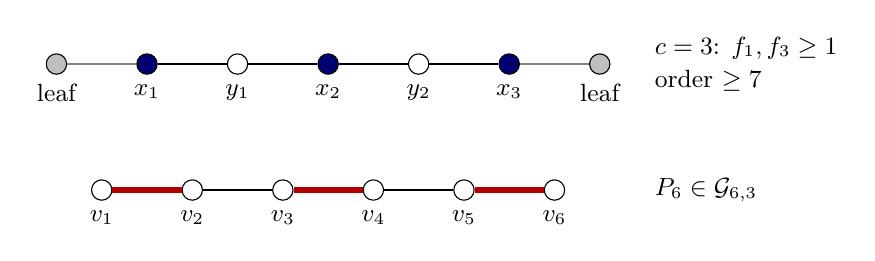
\begin{tikzpicture}[x=1.15cm,y=1cm,
  X/.style={circle,draw,fill=blue!45!black,inner sep=2.6pt},
  Y/.style={circle,draw,fill=white,inner sep=2.6pt},
  L/.style={circle,draw,fill=black!25,inner sep=2.6pt}]
  \node[L,label=below:{\small leaf}] (l1) at (0,0) {};
  \node[X,label=below:{\small $x_1$}] (a) at (1,0) {};
  \node[Y,label=below:{\small $y_1$}] (b) at (2,0) {};
  \node[X,label=below:{\small $x_2$}] (c) at (3,0) {};
  \node[Y,label=below:{\small $y_2$}] (d) at (4,0) {};
  \node[X,label=below:{\small $x_3$}] (e) at (5,0) {};
  \node[L,label=below:{\small leaf}] (l2) at (6,0) {};
  \draw (a)--(b)--(c)--(d)--(e); \draw[gray] (l1)--(a) (e)--(l2);
  \node[right,align=left] at (6.5,0) {\small $c=3$: $f_1,f_3\ge 1$\\ \small order $\ge 7$};
  \foreach \i in {1,...,6} \node[Y,label=below:{\small $v_{\i}$}] (p\i) at (\i-0.5,-1.6) {};
  \draw[line width=2.4pt,red!70!black] (p1)--(p2) (p3)--(p4) (p5)--(p6);
  \draw (p2)--(p3) (p4)--(p5);
  \node[right,align=left] at (6.5,-1.6) {\small $P_6 \in \G_{6,3}$};
\end{tikzpicture}
\caption{Top: Construction~9 with $k=3$, $n=6$ and $T_1$ the path $x_1x_2x_3$. The ends
need $f_1, f_3 \ge 1$, so the built tree has at least 7 vertices. The other tree on three
vertices is the same path with other labels. Bottom: the path $P_6$ with a perfect
matching (thick edges).}
\label{fig:example}
\end{figure}

\section{Proof of Theorem~\ref{thm:main}}

Let $k \ge 3$ and $n = 2k$. Write $d_i = d_{T_1}(x_i)$.

\begin{enumerate}
\item \emph{The value of $c$.} Here $c = \lfloor (4k-3)/k \rfloor$. Since $k \ge 3$, we have
$3k \le 4k-3 < 4k$, so $c = 3$.
\item \emph{One vertex.} The condition is $2d_i + f_i \in \{3,4\}$ with $d_i, f_i \ge 0$.
The solutions $(d_i, f_i)$ are $(0,3)$, $(0,4)$, $(1,1)$, $(1,2)$ and $(2,0)$. In each
solution, $d_i + f_i \ge 2$.
\item \emph{Sum over $X$.} So $\sum_i d_i + \sum_i f_i \ge 2k$. The tree $T_1$ has $k-1$
edges, so $\sum_i d_i = 2(k-1)$. Hence $\sum_i f_i \ge 2$.
\item \emph{Order.} Step~1 adds one vertex for each of the $k-1$ edges of $T_1$. Step~2
adds $\sum_i f_i$ leaves. So the built tree has
$k + (k-1) + \sum_i f_i \ge 2k+1$ vertices. \qed
\end{enumerate}

\begin{remark}[small $k$]
The condition $k \ge 3$ is necessary. For $k = 1$ and $n = 2$, $c = 1$, and $f_1 = 1$
gives $K_2 = P_2$. For $k = 2$ and $n = 4$, $c = 2$, $T_1 = K_2$ and $(f_1, f_2) = (1,0)$
give $P_4$. In both cases the path is in $\Tp_{2k,k}$, and our search confirms that it is
the minimiser.
\end{remark}

\begin{remark}[Construction 2]
When $k \mid (n-3)$, the family $\mathcal{T}_{n,k}$ of Construction~2 of \cite{HT} is the
part of $\Tp_{n,k}$ with $2d_i + f_i = c$ for all $i$. The only pair with $n = 2k$,
$k \ge 3$ and $k \mid (n-3)$ is $(n,k) = (6,3)$, so Theorem~\ref{thm:main} also shows that
$\mathcal{T}_{6,3}$ has no tree of order 6. This agrees with the remark in \cite{HT}
after Construction~2, which claims a member of $\mathcal{T}_{n,k}$ only for $k \ge 4$.
\end{remark}

\begin{remark}[ceiling]
The page image of \cite{HT} shows floor brackets around $(n+2k-3)/k$. With a ceiling
instead, $c = 3$ for $k = 3$, and $c = 4$ for $n = 2k$ and $k \ge 4$. In the second case
$f_i \ge 4 - 2d_i$, so $\sum_i f_i \ge 4k - 4(k-1) = 4$, and the built tree has at least
$2k+3$ vertices. The independent checker tests this reading too
(Section~\ref{sec:checks}). The conclusion does not change.
\end{remark}

\section{Computation}\label{sec:computation}

The minimisers of $\G_{n,k}$ are trees \cite{LLT}. So the program \texttt{checks/search.py}
takes every tree of order $n \le 20$ (generated by NetworkX \cite{nx}), computes its matching number
exactly and its spectral radius in floating point (NumPy \cite{nx}), and keeps, for each $k$, the
trees whose spectral radius is within $10^{-9}$ of the minimum. It then builds
$\Tp_{n,k}$ from every non-isomorphic tree $T_1$ on $k$ vertices and every admissible
$f$ with order $n$, and it tests each minimiser for membership by a canonical form of
the tree.

There are 100 pairs $(n,k)$ with $2 \le n \le 20$. The results are:
\begin{itemize}
\item For 8 pairs, a minimiser is outside $\Tp_{n,k}$. These are exactly the pairs
$(2k,k)$ with $k = 3,\dots,10$. In each of them $\Tp_{n,k}$ has no tree of order $n$, and
the unique minimiser is the path $P_{2k}$ (Table~\ref{tab:paths}).
\item For the other 92 pairs, every minimiser is in $\Tp_{n,k}$. These are the 90 pairs
with $n \ge 2k+1$ and the 2 pairs $(2,1)$ and $(4,2)$.
\item Four pairs have more than one minimiser within the tolerance: $(13,4)$ and $(17,4)$
with 3 trees, $(18,6)$ with 4 trees, and $(19,4)$ with 2 trees. All of them are in
$\Tp_{n,k}$.
\end{itemize}

\begin{table}[ht]
\centering
\begin{tabular}{rrrr}
\toprule
$k$ & $n=2k$ & trees built by Construction~9 of order $n$ & $\rho(P_{2k})$ \\
\midrule
3 & 6 & 0 & 1.801938 \\
4 & 8 & 0 & 1.879385 \\
5 & 10 & 0 & 1.918986 \\
6 & 12 & 0 & 1.941884 \\
7 & 14 & 0 & 1.956295 \\
8 & 16 & 0 & 1.965946 \\
9 & 18 & 0 & 1.972723 \\
10 & 20 & 0 & 1.977662 \\
\bottomrule
\end{tabular}
\caption{The 8 pairs $(n,k)$ with $n \le 20$ where a minimiser is outside $\Tp_{n,k}$.
In each, the unique minimiser in the search is $P_{2k}$, and its computed spectral radius
agrees with $2\cos(\pi/(2k+1))$ to within $10^{-9}$.}
\label{tab:paths}
\end{table}

These results are computed in floating point, with a tolerance for ties. They are
evidence, not a proof. The proof of Corollary~\ref{cor:answer} does not use them. They
support the following restricted question, which stays open.

\begin{question}
For $n \ge 2k+1$, must every spectrally minimal graph in $\G_{n,k}$ belong to $\Tp_{n,k}$?
\end{question}

That $P_n$ has the smallest spectral radius among connected graphs of order $n$ is
usually attributed to Collatz and Sinogowitz. We did not read their paper, and we do not
use this fact.

\section{How the result was checked}\label{sec:checks}

\paragraph{Lean.}
The file \texttt{lean/Solution.lean} states and proves Theorem~\ref{thm:main} in Lean~4
(v4.36.0) with Mathlib (tag v4.36.0) \cite{lean}. The statement, which \texttt{lean/Challenge.lean}
repeats with \texttt{sorry} as the proof, is:

\begin{lstlisting}
def Construction9Data (n k : (*@$\mathbb{N}$@*)) (T1 : SimpleGraph (Fin k)) [DecidableRel T1.Adj]
    (f : Fin k (*@$\to$@*) (*@$\mathbb{N}$@*)) : Prop :=
  T1.IsTree (*@$\wedge$@*) (*@$\forall$@*) i, 2 * T1.degree i + f i = (n + 2 * k - 3) / k (*@$\vee$@*)
    2 * T1.degree i + f i = (n + 2 * k - 3) / k + 1

def construction9Order (k : (*@$\mathbb{N}$@*)) (T1 : SimpleGraph (Fin k)) [DecidableRel T1.Adj]
    (f : Fin k (*@$\to$@*) (*@$\mathbb{N}$@*)) : (*@$\mathbb{N}$@*) :=
  k + #T1.edgeFinset + (*@$\sum$@*) i, f i

theorem construction9_no_tree_of_order_two_mul (k : (*@$\mathbb{N}$@*)) (hk : 3 (*@$\le$@*) k)
    (T1 : SimpleGraph (Fin k)) [DecidableRel T1.Adj] (f : Fin k (*@$\to$@*) (*@$\mathbb{N}$@*))
    (h : Construction9Data (2 * k) k T1 f) : construction9Order k T1 f (*@$\neq$@*) 2 * k
\end{lstlisting}

\noindent The match with Construction~9 is as follows. $X$ is \texttt{Fin k}, and
$T_1$ is a Mathlib simple graph on it with \texttt{IsTree}. The $f_i$ are natural numbers,
which include 0. On natural numbers, \texttt{/} is the floor of the quotient, and the
subtraction $n + 2k - 3$ is exact because $n + 2k \ge 3$. The order of the built tree is
the definition \texttt{construction9Order}: $|X|$, plus one vertex for each edge of $T_1$,
plus the leaves. Lean does not build the tree itself, and it does not define the matching
number, the spectral radius or $\G_{n,k}$. So Lean checks steps 1 to 4 of the proof for
all $k \ge 3$. The two facts in the proof of Corollary~\ref{cor:answer} (that $P_{2k}$ is
in $\G_{2k,k}$, and that a finite non-empty family has a minimiser) are checked by hand,
and by the Python checkers for small $k$.

The command \texttt{\#print axioms} gives
\[\texttt{[propext, Classical.choice, Quot.sound]}.\]
The proof uses no \texttt{native\_decide}. The \texttt{lake comparator} tool confirms
that \texttt{Solution.lean} proves exactly the theorem of \texttt{Challenge.lean}.

\paragraph{Python.}
Two checkers were written separately. They are not formally verified.
\begin{itemize}
\item \texttt{checks/verify.py} uses only the standard library and exact integers. For
$k = 3,\dots,8$ it takes the degree sequence of every labelled tree on $k$ vertices (from
all Pr\"ufer codes) and every admissible $f$, and it finds no order equal to $2k$. It
computes the matching number of $P_{2k}$ by brute force over all edge sets and gets $k$.
As a control, it finds members for $n = 2k+1$.
\item \texttt{checks/verifier\_check.py} builds every graph of Construction~9 explicitly
for $k = 3,\dots,7$, with both the floor and the ceiling reading of $c$. The smallest
order built is $2k+1$ (floor). For $k = 3,\dots,6$ it also takes every tree of order $2k$
with matching number $k$ and searches it for a set $X$ that shows it as a member of
$\Tp_{2k,k}$. It finds none, and the unique tree of minimum spectral radius is the path.
Controls: for $n = 2k+1$ the minimiser is a member, and $P_4 \in \Tp_{4,2}$.
\end{itemize}

\section{Limits}

\begin{enumerate}
\item The result is at the boundary $n = 2k$ of Construction~9. It shows that the stated
range of the construction is too large by one value of $n$ for $k \ge 3$. It gives no
information about the range $n \ge 2k+1$, which is the main content of the question.
\item The result answers the question as written in arXiv v1 and v2 of \cite{HT}. We did
not read the journal version \cite{HTj}. It is not confirmed that the journal version
keeps the range $n \ge 2k$.
\item Lean checks the counting step only. The membership $P_{2k} \in \G_{2k,k}$ and the
existence of a minimiser are elementary and are checked by hand.
\item The search of Section~\ref{sec:computation} uses floating point and a tolerance
for ties. Its statements about the pairs with $n \ge 2k+1$ are evidence only.
\end{enumerate}

\begin{thebibliography}{9}
\bibitem{HT} X. Hou, L. Tan, \emph{Tight lower bound for the spectral radius of connected
graphs with given matching number}, arXiv:2607.11061, v1 (13 July 2026) and v2
(17 July 2026). \url{https://arxiv.org/abs/2607.11061}
\bibitem{HTj} X. Hou, L. Tan, \emph{Tight lower bound for the spectral radius of
connected graphs with given matching number}, Linear Algebra Appl.\ 755 (2027) 151--163,
\href{https://doi.org/10.1016/j.laa.2026.10.032}{doi:10.1016/j.laa.2026.10.032}.
Bibliographic record checked in Crossref; full text not read.
\bibitem{LLT} J. Liu, Z. Lou, V. Trevisan, \emph{Minimal spectral radius of graphs with
given matching number}, arXiv:2601.18223 (2026), \url{https://arxiv.org/abs/2601.18223};
Linear Algebra Appl.\ 746 (2026) 88--110,
\href{https://doi.org/10.1016/j.laa.2026.05.011}{doi:10.1016/j.laa.2026.05.011}.
\bibitem{lean} The Lean~4 theorem prover, \url{https://github.com/leanprover/lean4}, and
the Mathlib library, \url{https://github.com/leanprover-community/mathlib4}.
\bibitem{nx} NetworkX 3.7, \url{https://networkx.org}, and NumPy 2.5.5,
\url{https://numpy.org}.
\end{thebibliography}

\end{document}
